\section{TICL Trackerster reconstruction after CLUE}
\label{sec:hgcal:reco}


% The CMS endcap calorimeter upgrade for the High Luminosity LHC in 2027 uses silicon sensors to achieve radiation tolerance, with the further benefit of a very high readout granularity. Small scintillator tiles with individual SiPM readout are used in regions permitted by the radiation levels. A reconstruction framework is being developed to fully exploit the granularity and other significant features of the detector like precision timing, especially in the high pileup environment of HL-LHC. 

% An iterative clustering framework (TICL) has been put in place, and is being actively developed. The framework takes as input the clusters of energy deposited in individual calorimeter layers delivered by the CLUE algorithm, which has recently been revised and tuned. Mindful of the projected extreme pressure on computing capacity in the HL-LHC era, the algorithms are being designed with modern parallel architectures in mind. Important speedup has recently been obtained for the clustering algorithm by running it on GPUs. Machine learning techniques are being developed and integrated into the reconstruction framework. This paper will describe the approaches being considered and show first results.



% The reconstruction software in HGCAL is being developed with speed and portability in mind. The expected CPU trend in the next years will improve software performance by a factor~$ \sim3$~\cite{4}, while offline workflows and computing in CMS will require a factor~$ \sim30$, mainly driven by the reconstruction of simulated events~\cite{5}. In order to gain the missing factor~$ \sim10$ in performance, the HGCAL software reconstruction cannot rely on any other existing sub-detector software: this new detector represents a unique opportunity to exploit modern architectures and technologies. Therefore, two main solutions are being adopted to provide the needed improvements in CMS performance for Phase-2 runs: heterogeneous computing and machine learning. On the hardware side, GPUs have shown great results in terms of speedup in recent years and the use of hybrid architectures is spreading in many fields of science. In addition, NVIDIA GPUs can be programmed with CUDA (Compute Unified Device Architecture), a parallel computing platform and programming model designed to work with programming languages such as C, C++, Fortran and Python, allowing to easily accelerate compute intensive portions of the applications~\cite{6}. On the software side, machine learning models are largely exploited to accomplish an enormous variety of tasks and can provide better results than traditional methods in many cases. Furthermore, some machine learning algorithms (e.g. Convolutional Neural Networks) can be executed on GPU, thus reducing both training and inference times, thanks to frameworks like Tensorflow~\cite{7} and Keras~\cite{8}.

% \subsection{TICL: The Iterative CLustering}
\noindent The development of the HGCAL reconstruction software is driven by three main concepts:

\begin{itemize}
    \item Particles deposit energy and create \emph{RecHits};
    \item \emph{RecHits} on each layer are clustered together to form \emph{LayerClusters} (2D objects);
    \item \emph{LayerClusters} are linked together to form \emph{Tracksters}, collections of \emph{LayerClusters}.
\end{itemize}

% In order to build the reconstruction chain exploiting the full potential of HGCAL, a modular framework has been developed and is constantly evolving. TICL (The Iterative CLustering)~\cite{9} modules and interfaces are defined such that new developers don't need a deep knowledge of the official CMS software core framework (CMSSW) and can easily contribute. In addition, its flexibility and modularity allow users to test their own algorithms and compare performances, as they can be plugged on top of the framework without applying any strong modification to the existing workflow. 

\noindent For \emph{LayerClusters}, the CLUE algorithm and its CMSSW application have been discussed in Section~\ref{sec:clue} and \ref{sec:cmsswClue}. Based on the \emph{LayerClusters} from CLUE, TICL framework is designed to link the \emph{LayerClusters} together to construct \emph{Tracksters} that representing particle flow candidates.
The design of TICL framework is shown in Figure~\ref{fig:ticl}. This section focuses on the two main aspects of TICL reconstruction. First, a typical TICL iteration that links \emph{LayerClusters} together to produce \emph{Tracksters} will be described in Section~\ref{sec:iter}.  Second, the preliminary results of particle identification and energy regression performed on a \emph{Trackster} with a Convolutional Neural Network are shown in Section~\ref{sec:pid}.

\begin{figure}[tbp]
    \centering % \begin{center}/\end{center} takes some additional vertical space
    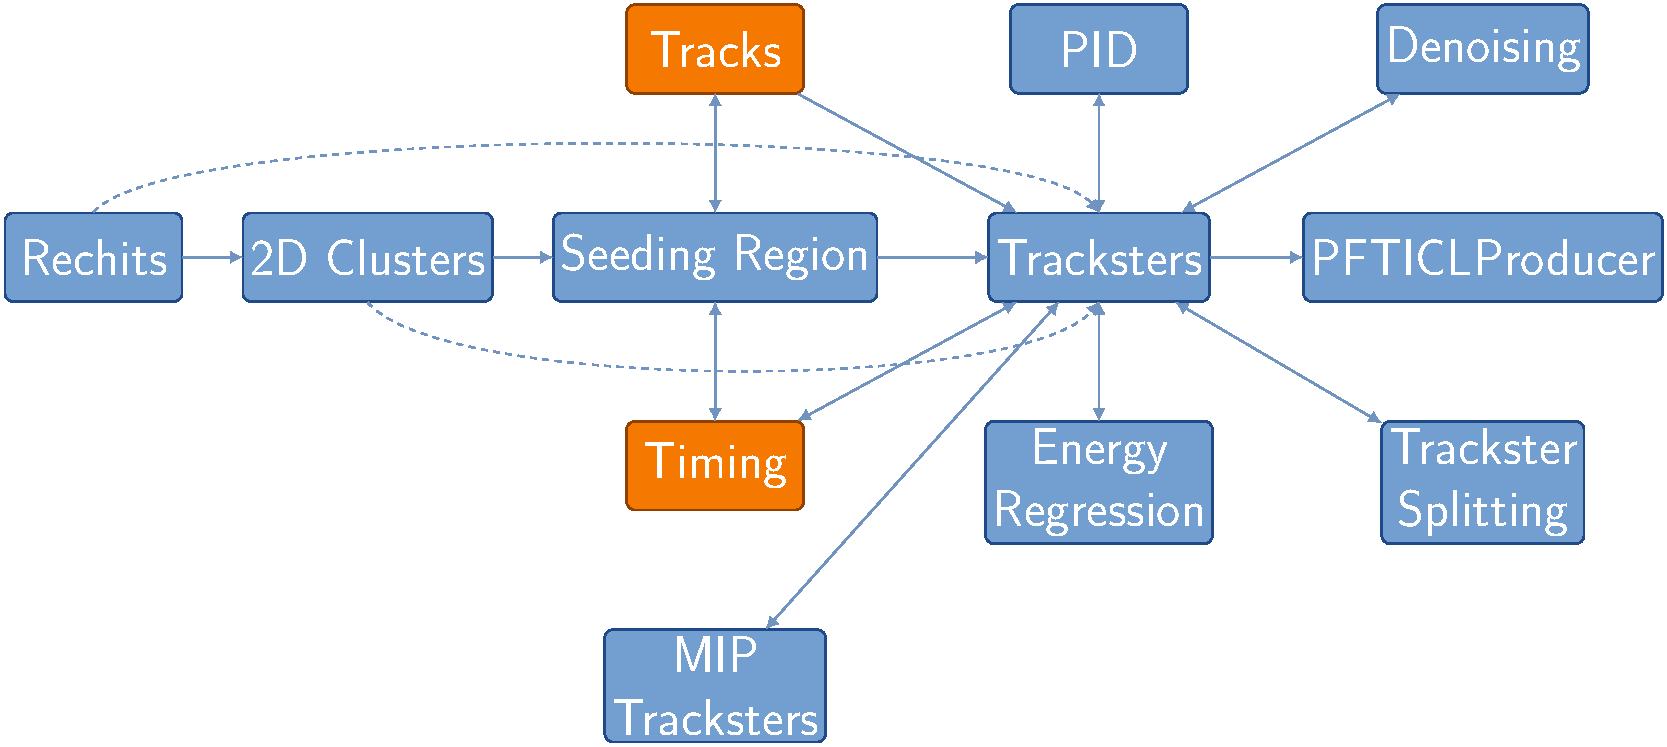
\includegraphics[width=.9\textwidth]{chapters/HGCal/figures/chef/ticl.pdf} 
    \caption{\label{fig:ticl} Design of TICL framework. Arrows show connections between different parts of the reconstruction, pointing from the output of a step to the input of a next step. Double pointing arrows indicate a strong connection between two parts of the reconstruction. \emph{Tracks} and \emph{Timing} (orange cells) are information coming from other subdetectors (respectively Tracker and MTD)~\cite{ticlwebsite}.}
\end{figure}


\subsection{Iterations}
\label{sec:iter}

\emph{Tracksters} produced by TICL iterations are suitable for representing real physics objects (i.e. particle showers). In order to guarantee such a correspondence, it's necessary to build a reconstruction workflow that takes into account the specific physics process that different particles undergo into the detector (hadronic and electromagnetic shower development, minimum ionizing particles, e.g. muons, etc.). Four different types of iteration exist now in TICL: \emph{track-seeded} (collects information from the Tracker to get the entry point and momentum direction of charged particles at the front face of the HGCAL detector), \emph{MIP} (\emph{Minimum Ionizing Particle}), \emph{electromagnetic} and \emph{hadronic}. The structure of a TICL iteration is shown in Figure~\ref{fig:iter}. A seeding region is first defined as a window in the [$\eta$, $\phi$] space on a certain layer and a pattern recognition algorithm is applied to all the available \emph{LayerClusters} within the seeding region. Then, linking, cleaning and classification tasks follow, exploiting timing information when possible. At the end of each iteration, the \emph{Tracksters} are required to pass quality criteria and particle identification: all the \emph{LayerClusters} belonging to the selected \emph{Tracksters} are masked out and are not available for the next iteration.

\begin{figure}[tbp]
    \centering % \begin{center}/\end{center} takes some additional vertical space
    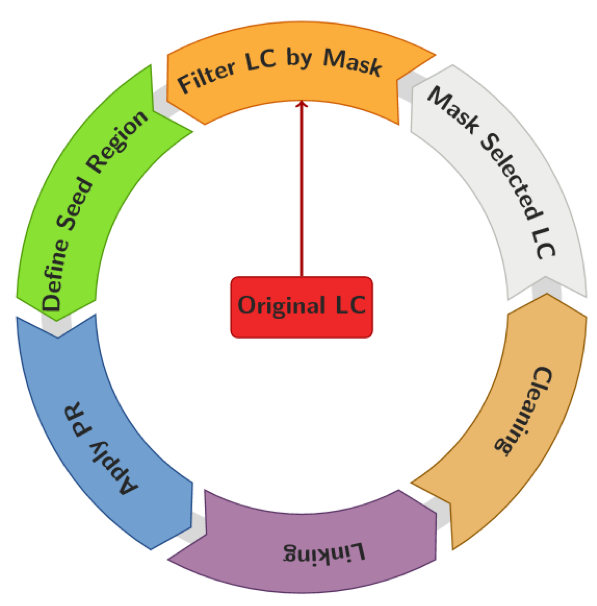
\includegraphics[width=.4\textwidth]{chapters/HGCal/figures/chef/iter}
    \qquad
    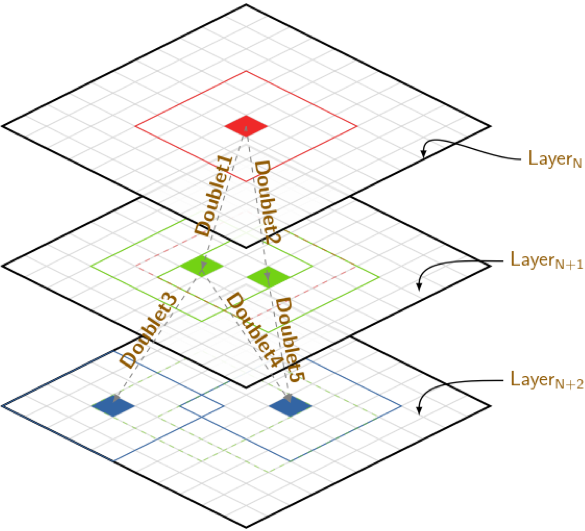
\includegraphics[width=.4\textwidth]{chapters/HGCal/figures/chef/pralgo}
    % "\includegraphics" from the "graphicx" permits to crop (trim+clip)
    % and rotate (angle) and image (and much more)
    \caption{\label{fig:iter} (\emph{Left}) Structure of a typical iteration in TICL. (\emph{Right}) Scheme of \emph{Cellular Automaton} pattern recognition implemented in TICL~\cite{ticlwebsite}.}
\end{figure}

Thanks to the modular design of the framework, several pattern recognition algorithms can be tested to produce the best results. Currently, a \emph{Cellular Automaton} algorithm is being used based on the experience with CMS Track reconstruction~\cite{Funke:2014dga}. It consists of six main steps:

\begin{enumerate}
\itemsep0em
    \item Start from a Layer\textsubscript{N} and consider a specific \emph{LayerCluster}
    \item Open a window in the [$\eta$, $\phi$] space around it and project it onto the next Layer\textsubscript{N+1}
    \item Consider all the \emph{LayerClusters} inside this region and try to establish a \emph{Doublet} connection between the \emph{LayerClusters} on the two adjacent layers
    \item Apply some compatibility criteria to decide if the \emph{LayerClusters} should be linked or not (i.e. geometry constraints, energy, timing compatibility, etc.)
    \item Repeat this same procedure for all the \emph{LayerClusters} on Layer\textsubscript{N}
    \item Repeat this same procedure for all pairs of contiguous layers [Layer\textsubscript{K}, Layer\textsubscript{K+1}]
\end{enumerate}

At the end of the process, pairs of \emph{LayerClusters} will be connected into \emph{Doublets}. Consecutive \emph{Doublets} (i.e. doublets that share the ``middle'' \emph{LayerCluster}) will be linked together if configurable alignment requirements are satisfied. The set of all connected \emph{Doublets} will form a direct acyclic graph that serves as building block for a \emph{Trackster}. Note that this procedure can be properly configured to allow missing consecutive \emph{LayerClusters} and establish links between non-adjacent layers (e.g. in \emph{MIP} iteration). 





\subsection{Particle identification and energy regression}
\label{sec:pid}
The final purpose of the TICL is to reconstruct particle-flow objects with energies and probabilities of particle identification. To accomplish this task, some preliminary studies were conducted with a single particle produced in front of HGCAL in events where no pile-up is simulated. The momentum of the particle pointed from the vertex (0,0,0), center of the CMS detector. Events were simulated in such a way that particle showers (in case of electrons, photons and charged hadrons) could be fully contained inside the detector.

Since \emph{Tracksters} are suitable for representing real physics objects, a Convolutional Neural Network was designed to perform particle identification and energy regression on \emph{Tracksters} built by TICL electromagnetic iterations. In order to have fixed-sized inputs to the network, each \emph{Trackster} is represented as an image $50 \times 10 \times 3$, where the dimensions represent respectively the number of HGCAL layers per endcap, the maximum number of \emph{LayerClusters} on each layer and the number of features (energy, $\eta$, $\phi$). In this representation, each pixel of the image corresponds to a \emph{LayerCluster} that belongs to the \emph{Trackster}. Furthermore, \emph{LayerClusters} on each layer have been sorted by decreasing energy, applying a zero-padding whenever a layer featured less than 10 clusters, while removing some low energy \emph{LayerClusters} in layers with more than 10.

\begin{figure}[t]
    \centering
    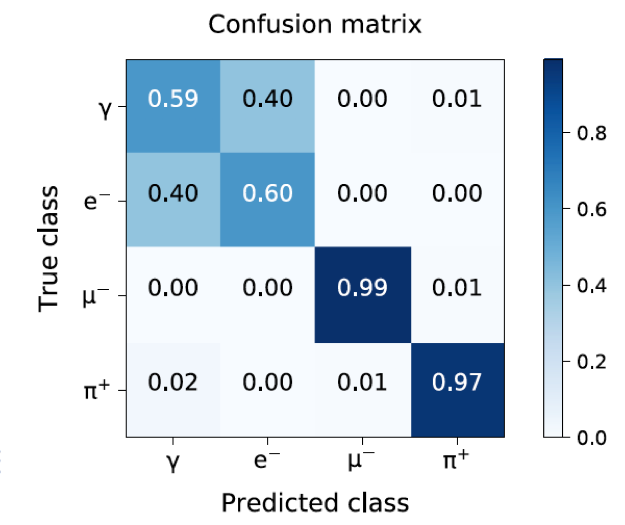
\includegraphics[width=.4\textwidth]{chapters/HGCal/figures/chef/pid}
    \caption{\label{fig:pid} Confusion matrix showing the performance of particle identification.}
\end{figure}

\begin{figure}[h]
    \centering
    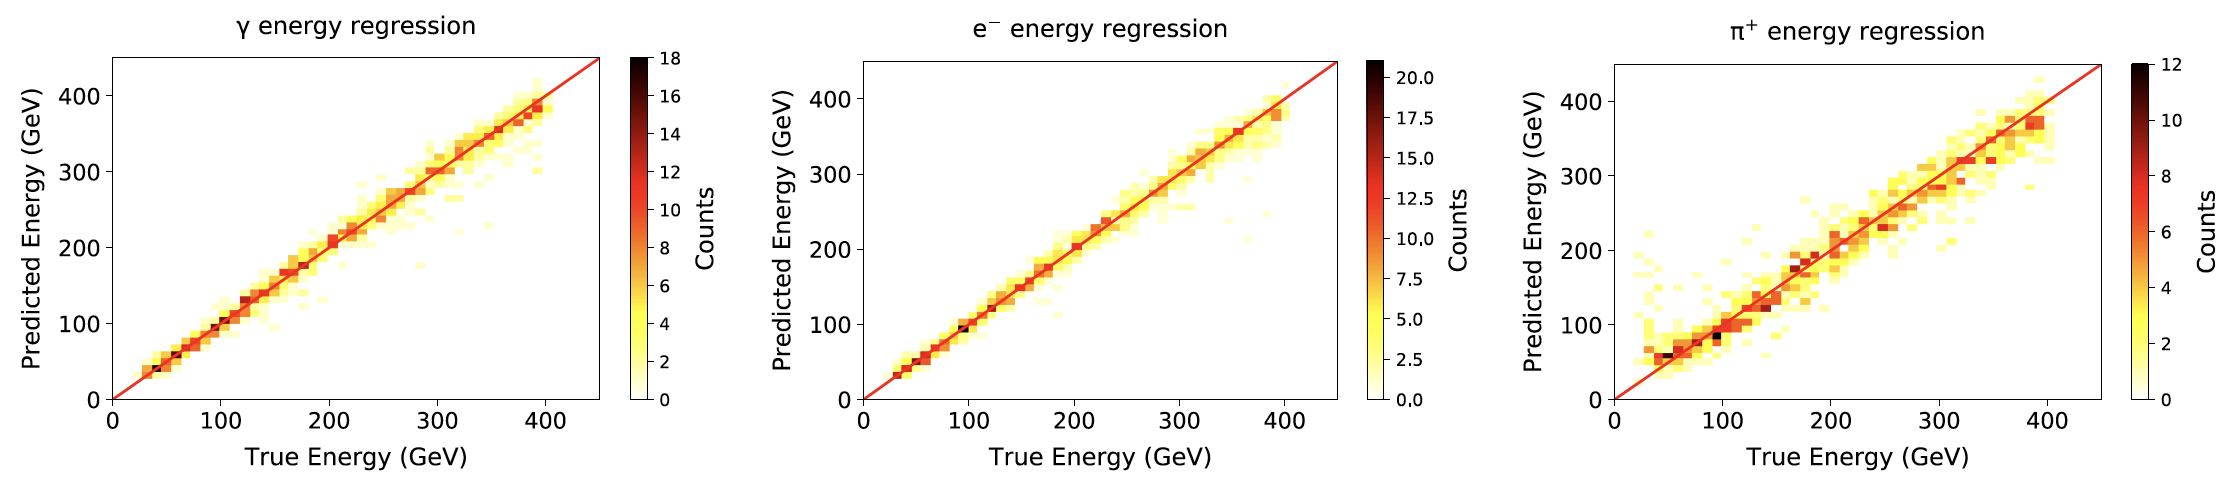
\includegraphics[width=.99\textwidth]{chapters/HGCal/figures/chef/er}
    \caption{\label{fig:er} Energy regression preliminary results for photons, electrons and charged hadrons.}
\end{figure}

A preliminary performance study was conducted on a 4-classes model (electron, photon, muon, charged hadron). The dataset consisted of 40 thousand events (10 thousand per particle type): $80\%$ has been used for training, $10\%$ for validation and the remaining $10\%$ for testing. The CNN was trained for 15 epochs (passes of the algorithm through the entire dataset), using the sum of cross-entropy and mean squared error as loss function to account for particle ID and energy regression, respectively. In order to have the value of the two functions of the same order of magnitude during training, the energies of the \emph{Tracksters} were normalized with respect to the data sample. The CNN was trained with Tensorflow~\cite{tensorflow2015-whitepaper}. Results are shown in Figure~\ref{fig:pid} and Figure~\ref{fig:er}. The confusion between electrons and photons is expected to be solved in future by exploiting information coming from the Tracker. The energy regression must be fine tuned and improvements are needed especially in the case of charged hadrons, since part of the shower is reconstructed by hadronic iteration. More classes will be added and the evolution of TICL is expected to improve the performance of this task.

